\documentclass{beamer}

\AtBeginSubsection[]
{
\begin{frame}<beamer>
\frametitle{Outline}
\tableofcontents[
  currentsection,
  sectionstyle=show/hide,
  subsectionstyle=show/shaded/hide
]
\end{frame}
}

\usepackage[francais]{babel}
\usepackage[utf8x]{inputenc}
\usepackage[T1]{fontenc}
\mode<presentation> {

% The Beamer class comes with a number of default slide themes
% which change the colors and layouts of slides. Below this is a list
% of all the themes, uncomment each in turn to see what they look like.

%\usetheme{default}
%\usetheme{AnnArbor}
%\usetheme{Antibes}
%\usetheme{Bergen}
%\usetheme{Berkeley}
%\usetheme{Berlin}
%\usetheme{Boadilla}
%\usetheme{CambridgeUS}
%\usetheme{Copenhagen}
%\usetheme{Darmstadt}
%\usetheme{Dresden}
%\usetheme{Frankfurt}
%\usetheme{Goettingen}
%\usetheme{Hannover}
%\usetheme{Ilmenau}
%\usetheme{JuanLesPins}
%\usetheme{Luebeck}
\usetheme{Madrid}
%\usetheme{Malmoe}
%\usetheme{Marburg}
%\usetheme{Montpellier}
%\usetheme{PaloAlto}
%\usetheme{Pittsburgh}
%\usetheme{Rochester}
%\usetheme{Singapore}
%\usetheme{Szeged}
%\usetheme{Warsaw}

% As well as themes, the Beamer class has a number of color themes
% for any slide theme. Uncomment each of these in turn to see how it
% changes the colors of your current slide theme.

%\usecolortheme{albatross}
%\usecolortheme{beaver}
%\usecolortheme{beetle}
%\usecolortheme{crane}
%\usecolortheme{dolphin}
%\usecolortheme{dove}
%\usecolortheme{fly}
%\usecolortheme{lily}
%\usecolortheme{orchid}
%\usecolortheme{rose}
%\usecolortheme{seagull}
%\usecolortheme{seahorse}
%\usecolortheme{whale}
%\usecolortheme{wolverine}

%\setbeamertemplate{footline} % To remove the footer line in all slides uncomment this line
%\setbeamertemplate{footline}[page number] % To replace the footer line in all slides with a simple slide count uncomment this line

%\setbeamertemplate{navigation symbols}{} % To remove the navigation symbols from the bottom of all slides uncomment this line
}

\usepackage{graphicx}
\graphicspath{ {img/} }
\usepackage{booktabs}
\newsavebox{\longestsec}% Box to save longest sectional heading
\title[Exploitation binaire]{Exploitation binaire : Une introduction (1/2)}

\author{Frédéric Vachon}
 
\date{\today}

\begin{document}

\begin{frame}
\titlepage
\end{frame}

\begin{frame}[plain,c]
\frametitle{Plan de la présentation}
\tableofcontents
\end{frame}

\section{Assembleur x86}


\subsection{Mémoire}


\begin{frame}{\insertsection: \insertsubsection}
  \centering
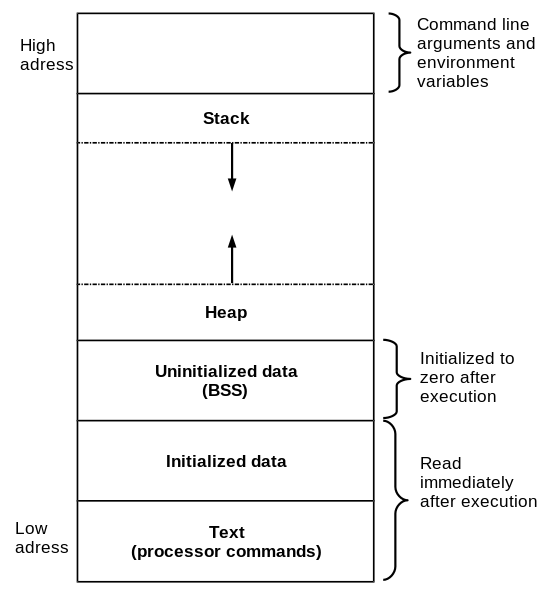
\includegraphics[scale=0.35]{memlayout}

\end{frame}

\subsection{Registres}


\subsection{Instructions}


\section{Du C vers l'assembleur}

\subsection{Cadres d'activation (stack frame)}

\subsection{Appels de fonctions}

\subsection{Conditions}

\section{Buffer overflow et Exploitation}
\subsection{Fonctions vulnérables}
\subsection{Changer une variable sur la pile}
\subsection{Contrôler l'adresse de retour}
\subsection{Injection et exécution d'un shellcode}

\section{Débogguage Bas Niveau}

\begin{frame}
  salut
  \end{frame}


\end{document}